%----------------------------------------------------------------------------------------
%	PACKAGES AND THEMES
%----------------------------------------------------------------------------------------

\documentclass[notes]{beamer}

%Cheat-Sheet: https://www.cpt.univ-mrs.fr/~masson/latex/Beamer-appearance-cheat-sheet.pdf
\usetheme{Frankfurt}

%-- Layout --%
% font size
\usepackage[fontsize=11pt]{scrextend}
\usepackage{amsmath}
\usepackage[short]{optidef}
\usepackage[backend=bibtex,style=authoryear]{biblatex}
% page
\setbeamersize{text margin left=1cm, text margin right=1cm}
\setbeamercolor{button}{bg=blue, fg=white}
% line space 
% footline
\addtobeamertemplate{navigation symbols}{}{
    \usebeamerfont{footline}
    % \usebeamercolor[fg]{footline}
    \hspace{2em}
    \insertframenumber/\inserttotalframenumber    }
% headline
\setbeamercovered{transparent}

%-- Figure --%
\usepackage{graphicx}
% \usepackage{subfig}

%-- Table --%
\usepackage{tabularx,booktabs}
\newcolumntype{Y}{>{\centering\arraybackslash}X}

%-- Text --%
\usepackage{xcolor}
% \usepackage{tikz}

%-- Math --%
\usepackage{amssymb}
\usepackage{amsmath}

%-- Caption --%
\usepackage{caption}
\usepackage{subcaption}

%-- Effects --%
\usepackage{hyperref}

% !TEX program = pdflatex
% !TEX enableSynctex = true
% !BIB program = bibtex


%----------------------------------------------------------------------------------------
%	TITLE PAGE
%----------------------------------------------------------------------------------------

\title[]{The Nature of Corporate Credit Constraints} % The short title appears at the bottom of every slide, the full title is only on the title page

\author{Barnab\'as Sz\'ekely} % Your name

\date{\today } % Date, can be changed to a custom date

\begin{document}
\renewcommand{\arraystretch}{1.4}

\begin{frame}
\titlepage % Print the title page as the first slide
\end{frame}

%%----------------------------------------------------------------------------------------
%	PRESENTATION SLIDES
%----------------------------------------------------------------------------------------

%------------------------------------------------
\section{Introduction}

\begin{frame}[label=intro1] \frametitle{Credit market frictions in macro-finance}
Asset-based constraints
\begin{itemize}
 \setlength\itemsep{0em}
    \item Underlying debt contract: \textbf{asset-based}
    \item Backed by physical assets, in-default payments are expected from liquidation of the collateral
\end{itemize} 

Earnings-based constraints
\begin{itemize}
 \setlength\itemsep{0em}
    \item Underlying debt contract: \textbf{cash flow-based}
    \item Backed by future cash flows (not secured by specific assets) 
    \item In-default payments are expected after reorganization
    \item Lian and Ma (2021): 80\% of US corporate debt is CF-based
\end{itemize} \vspace{1mm}
\begin{center}
\hyperlink{secUnsec}{\beamerbutton{Secured vs. Unsecured}} 
\end{center}
\end{frame}

%------------------------------------------------
\begin{frame}[label=slide2] \frametitle{Reconsidering credit market frictions}

New contributions: consider EBCs instead of ABCs 
\begin{itemize}  \setlength\itemsep{0em}
    \item Significant effects on structural models
    \item Drechsel (2023), Lian and Ma (2021), Greenwald (2019)
\end{itemize} \vspace{1mm} \\
However, neither constraint describes credit frictions accurately!
\begin{itemize}  \setlength\itemsep{0em}
    \item Most firms hold asset-based and CF-based debt simultaneously
    \item These face some combination of the two frictions 
\end{itemize} \vspace{1mm} \\
Research question(s): 
\begin{itemize}
 \setlength\itemsep{0em}
    \item How firms utilize asset-based and CF-based debt finance?
    \item Implied credit frictions given firm characteristics?
    \item What are the aggregate effects of such frictions?
\end{itemize}

\end{frame}

\section{Empirics}

%------------------------------------------------
\begin{frame}[label=slide2] \frametitle{Data and Motivation}
Compustat and Capital IQ data; US traded firms; 2010-2023
\begin{itemize}  \setlength\itemsep{0em}
    \item Classification based on Lian and Ma (2021)
    \item Most firms typically hold multiple debt contracts (5.21 on average) and use on both type of debt!
\end{itemize} \vspace{0.1mm} \\
\begin{table}[h!]
\centering
\resizebox{0.95\textwidth}{!}{% 0.75 times the text width
\begin{tabular}{l|rrr|r}
\multicolumn{5}{l}{\textbf{Firm shares by debt financing strategy}} \\
\toprule
\textbf{Share by} & \textbf{\# of Firms} & \textbf{Assets}  & \textbf{Borrowing} &\\  
Asset-based firms & 35.66\% & 4.83\% & 3.36\% & AB frictions \\ 
'Hybrid' firms & 52.11\% & 87.27\% & 90.31\% & Combination \\ 
CF-based firms & 12.23\% & 7.91\% & 6.33\% & EB frictions \\ 
\bottomrule
\end{tabular}
}
\label{tab:shares}
\end{table} 

\begin{center}
\hyperlink{Classification}{\beamerbutton{More on classification}}
\hspace{2cm}
\hyperlink{distrib}{\beamerbutton{Class size distributions}}
\end{center}

\end{frame}

%------------------------------------------------
\begin{frame}[label = nameit] \frametitle{CFL reliance}
Define, \\
\begin{center}
    \text{CFL  reliance = CF-based debt / Total debt}
\end{center}
\vspace{3mm} \\
The main determinants of CFL reliance
 \begin{itemize}
     \setlength\itemsep{0em}
        \item Total assets (size) - U-shape
        \item Leverage - positive association
        \item Asset pledgeability - negative association
        \item Large fixed costs of lending against future cash-flows!
 \end{itemize} \vspace{3mm} \\

\begin{center}
\hyperlink{multi}{\beamerbutton{Multivariate Analyses}}
\hspace{2cm}
\hyperlink{fc}{\beamerbutton{Fixed costs}}
\end{center}

 
\end{frame}


%------------------------------------------------
\begin{frame}[label=slide3] \frametitle{CFL reliance - observations to match}
\begin{figure}[H]  % [h] indicates placing the image here
    \centering
    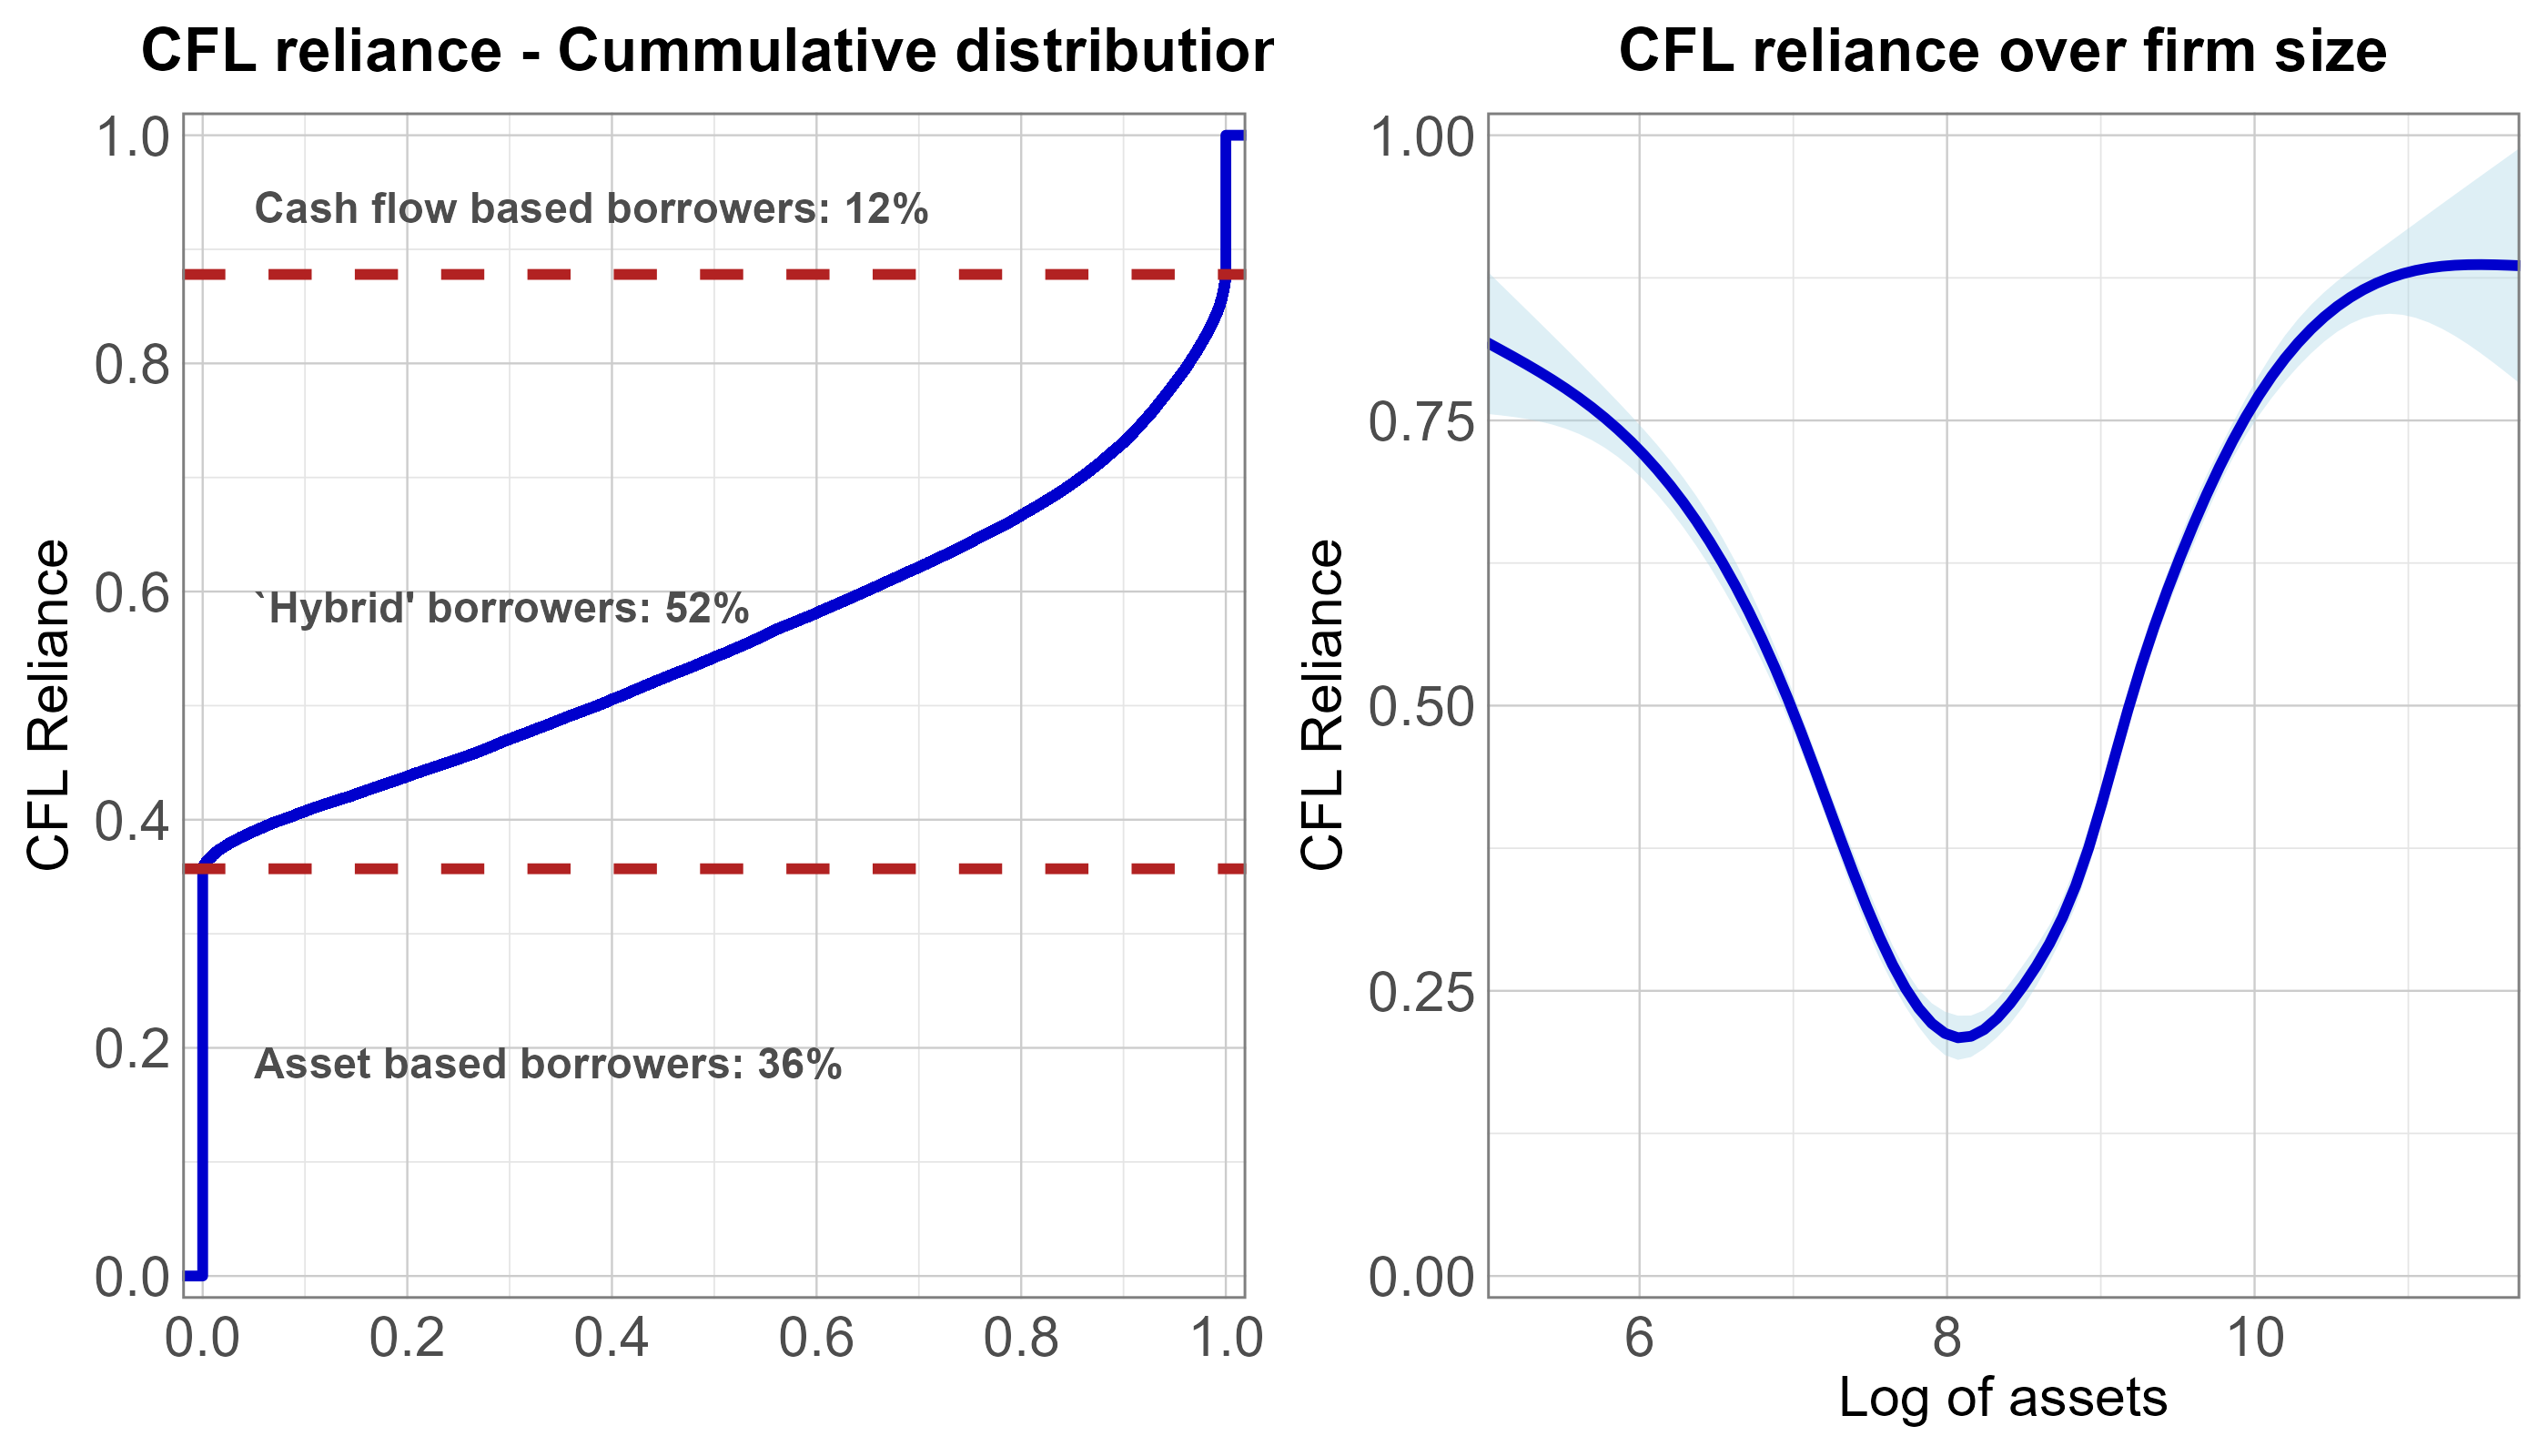
\includegraphics[width=1\textwidth]{smoothcfd.png}
\end{figure}
\begin{center}
\hyperlink{U_sector}{\beamerbutton{U-shape across sectors}}
\hspace{2cm}
\hyperlink{U_country}{\beamerbutton{U-shape across countries}}
\end{center}
\end{frame}

\section{Model}

%------------------------------------------------
\begin{frame}
\frametitle{Model preview}

Describing credit frictions given firm characteristics \vspace{1mm }\\
\hspace{2mm} $\leftarrow$  Firms' optimal debt financing strategy (CFL reliance) \vspace{1mm }\\
\hspace{2mm} $\leftarrow$  External finance premium under each debt contract \vspace{1mm }\\
\hspace{2mm} $\leftarrow$  \textbf{Lenders' expected costs and payoffs under ABL and CFL} \vspace{5mm }\\

Not (!) the goal: 
\begin{itemize} \setlength\itemsep{0em}
    \item Complete description of bankruptcy procedures
    \item Overview of various types of debt constructs
\end{itemize}

\end{frame}


%------------------------------------------------
\begin{frame}[label = HH]
\frametitle{Households}
Two types of agents: 
\begin{itemize} \setlength\itemsep{0em}
    \item Representative household
    \item Heterogeneous firms 
\end{itemize} \vspace{3mm} \\
Representative household:
\begin{itemize}\setlength\itemsep{0em}
\item Chooses consumption, labour and bonds
\item Holds non-contingent bonds $B$ at a gross interest rate: $1/q_0$
\item Owns firms
\end{itemize} 
\vfill % Add vertical space to push the button to the bottom
\begin{center}
\hyperlink{HH problem}{\beamerbutton{Household problem}}
\end{center}
 
\end{frame}

%------------------------------------------------
\begin{frame}
\frametitle{Firms}
Heterogeneous firms
\begin{itemize}  \setlength\itemsep{0em}
\item Heterogeneous productivity: $\varepsilon$ is a Markov chain
\item Accumulate capital $k$ and may borrow or save $b$
\item Subject to fixed costs of production and default shocks
\end{itemize} \vspace{3mm} \\
Maximize the discounted sum of dividends by choosing
\begin{itemize}  \setlength\itemsep{0em}
    \item current employment,    
    \item future capital stock, 
    \item future debt,
    \item debt financing strategy.
\end{itemize} 

\end{frame}

%------------------------------------------------
\begin{frame}[label = exdef]
\frametitle{Exogenous defaults}

Cash on hand, $x$: 
\begin{itemize}\setlength\itemsep{0em}
    \item A firm can be described by $(k,b,\varepsilon)$
    \item No adjustment costs, $k$ and $b$ is summarized in $x$
\end{itemize}  \vspace{2mm} \\

Default shocks:
\begin{itemize} \setlength\itemsep{0em}
\item Exogenous, uniformly distributed with probability $P_\chi$
\item Associated with zero value - continuation is discounted
\item Adds equilibrium defaults and lending risks
\end{itemize} \vspace{2mm} \\

Voluntary exit: 
\begin{itemize}
    \item Firms may also decide to exit - firm gets liquidated
\end{itemize}

\begin{center}
\hyperlink{volex}{\beamerbutton{Voluntary exit decision}}
\end{center}

\end{frame}

%------------------------------------------------
\begin{frame}[label = timing]
\frametitle{Model timing}
\textbf{T0 begins}
\begin{itemize} \setlength\itemsep{0em}
    \item Firms choose labour demand, produce, profits are realized and capital depreciates
    \item Default shocks materialize
    \item \textit{In default}: firms are reorganized or liquidated
    \begin{itemize}
        \item Asset-based contract: always liquidated
        \item Hybrid contract: the lender makes the reorg. decision
    \end{itemize}
    \item \textit{No default}: voluntary exit decision 
    \item Entrants enter as continuing firms
    \item Continuing firms choose debt financing strategy, future debt and capital
\end{itemize}
\textbf{T1 begins}

\end{frame}


%------------------------------------------------
\begin{frame}
\frametitle{Defaults and firm values}
Value of a continuing firm: 
\begin{equation*} \label{eq:V_2}
V_2(x,\varepsilon_i) = \max_{k',b', s \in \{A,H\}} \left(x - k' +  q^s(k',b',\varepsilon_i)b' + \beta \sum_{j=1}^{N_\varepsilon} g_{ij} V_0(x',\varepsilon_j') \right)
\end{equation*} 
subject to: 
\begin{equation*} \label{eq:cont_1}
x' = \pi(k',\varepsilon_j')+(1-\delta)k'-b'
\end{equation*}
$$ x - k' +  q^s(k',b',\varepsilon_i)b' \geq 0 $$\vspace{0.1mm} \\
External finance premium:
\begin{itemize}
    \item for a unit of debt, the lender provides $q^s$ units of output 
\end{itemize}

\end{frame}

%------------------------------------------------
\begin{frame}[label=slide2] \frametitle{Choosing debt financing strategy}
\begin{table}[h!]
\centering
\resizebox{1\textwidth}{!}{% 0.75 times the text width
\begin{tabular}{l|cc}
\textbf{Firms choose:}  & Asset based contract & Hybrid contract  \\  
  \midrule
Implied interest rate & $q^A(k',b')$ &  $q^H(k',b',\varepsilon_i)$ \\
CFL reliance & $0$ & $(0,1]$ \\ 
Default resolution & Liquidation & Liquidation \textbf{or} Reorganization \\ 
In-default payment & Value of assets & Value of assets \textbf{or} Cont. value\\ 
Fixed costs & Zero & Significant ($\zeta_1$, $\zeta_2$) \\
\bottomrule
\end{tabular}
}
\label{tab:shares}
\end{table}  \vspace{3mm} \\

Debt financing choice only affects current interest rate
\begin{itemize} \setlength\itemsep{0em}
    \item Firms consider: $q^A(k',b') \lessgtr q^H(k',b',\varepsilon_i)$ 
    \item Defined by lenders' costs and in-default payoffs
\end{itemize}

\end{frame}



%------------------------------------------------
\begin{frame}[label=exprem] \frametitle{External finance premium: asset based contracts ($q^{A}$)}
Asset-based lending: 
\begin{itemize} \setlength\itemsep{0em}
\item In default, the lender seizes the capital and re-sells it
\item Debt is backed only by the liquidation value of assets
\item In default payoff:  $ \phi_k (1-\delta) k'$
\end{itemize}  \vspace{5mm} \\
From zero profit condition: 
$$ q^A(k',b')b' = \beta \left[ (1-P_\chi) b' + P_\chi \min\{b', \ \phi_k (1-\delta) k' \} \right]    $$  

\end{frame}

%------------------------------------------------
\begin{frame}[label=hybrid] \frametitle{External finance premium: hybrid contracts ($q^{H})$}

Hybrid lending: 
\begin{itemize} \setlength\itemsep{0em}
    \item The lender decides between reorganization or liquidation
    \item Under reorganization the lender retrieves some fraction $\phi_v$ continuation value
\end{itemize}
From zero profit condition
\begin{equation*}
    \resizebox{1\hsize}{!}{$
    q^H(k',b',\varepsilon_i)b' = \beta \left[ (1-P_\chi) b' + P_\chi \sum_{j=1}^{N_\varepsilon} g_{ij}  \min\{b', \ \phi_v E[V^D_1(k',b',\varepsilon)]  \} - \zeta_2 \right]
    $}
\end{equation*}
where 
$$V_1^D(k,b,\varepsilon_i) = \max \Big\{ \phi_vV_2(k,b,\varepsilon_i)- \zeta_1, \  \phi_k (1-\delta) k \Big\}.$$
and $\zeta_1$ is reorganization costs and $\zeta_2$ is monitoring costs
\begin{center}
\hyperlink{fc}{\beamerbutton{Fixed costs}}
\hspace{10mm}
\hyperlink{assumpt}{\beamerbutton{Simplifying assumptions}}
\end{center}
\end{frame}


%------------------------------------------------
\begin{frame}[label=CFLrel] 
\frametitle{CFL reliance}
Extent to which 'hybrid' debt is backed by cash-flows: 
$$ \text{CFL reliance}  = \text{Pr(reorg.)} = \sum_{j = 1}^{N_\varepsilon} g_{ij} \left[ 1-\chi_1^D(k',b',\varepsilon_j')\right]  $$
$\chi_1^D = 1$ if the firm is liquidated under financial distress

\vfill

\begin{center}
\hyperlink{intuition}{\beamerbutton{Further intuition}}
\end{center}

\end{frame}


%------------------------------------------------

\begin{frame}[label=market clearing]{Stationary equilibrium}
Described by the set of functions  
$$(\mu, w, V_0, V_1, V_1^D, V_2, \chi^0, \chi^1, \chi^2,  \chi^e,  \chi^l, l,q^s,k,b,d, V_h, C, N, B)$$
such that: 
\begin{enumerate}[i]
\item Firms and the household maximize value 
\item Labour market clears: 
$ N = \int n  \ d \mu (x,\varepsilon)  $
\item Financial market clears:
$ B = \int b \ d \mu (x,\varepsilon) $
\item Goods market clear: 
$ C + I = \int y \ d \mu (x,\varepsilon)$
where: 
\begin{equation*}
    \resizebox{1\hsize}{!}{$
    I = \int (1-\chi_l)\left[ k' -(1-\delta)k \right] d \mu (x,\varepsilon) - \int \chi_l (1-\delta) k \ d \mu (x,\varepsilon)  + M \int \chi_e k \ d \Phi(x,\varepsilon) 
    $}
\end{equation*}
\item Firms distribution is stationary, $\Gamma(\mu) = \mu$ and prices $(w,q)$ are constant over time
\end{enumerate}

\end{frame}

\section{Conclusion}

\begin{frame}[label=concl] 
\frametitle{Conclusion, next steps}
Motivating evidence
\begin{itemize} \setlength\itemsep{0em}
    \item Most firms hold asset-based and CF-based debt simultaneously
    \item Face a combination of asset-based and earnings-based frictions
    \item Overlooked by previous analyses
\end{itemize}
Proposed model: 
\begin{itemize} \setlength\itemsep{0em}
    \item Firms react to the debt schedules $q^A(k',b')$ and $q^H(k',b',\varepsilon)$
    \item Reproduces CFL reliance across firms $\rightarrow$ more accurate description of credit frictions
\end{itemize}
Further steps
\begin{itemize} \setlength\itemsep{0em}
    \item Solve PE model for CFL reliance and integrate it in a GE setup
\end{itemize}

\end{frame}

\section{Appendix}


%------------------------------------------------
\begin{frame}[label=secUnsec] \frametitle{Secured vs. Unsecured lending}
Lian and Ma (2021): security is about priority in bankruptcy, not the economic determinants of creditors' pay-offs \vspace{3mm} \\
Correlated concepts:
\begin{itemize}
\item Unsecured debt it is CFL
\item Secured debt can still be CFL - if secured against the entire corporate entity (substantially all assets) or against equity
\item Lian and Ma: secured bonds typically fall to the latter category, they classify these as CFL 
\end{itemize}

\begin{center}
\hyperlink{intro1}{\beamerreturnbutton{back}}
\end{center}

\end{frame}

%------------------------------------------------
\begin{frame}[label=Classification] \frametitle{Classification details}
Main organizing principle: cash flow-based debt is not secured against any specific physical asset \vspace{4mm} \\
ABL debt: 
\begin{itemize}
 \setlength\itemsep{0em}
\item Mortgage bonds and notes, Commercial mortgages
\item Capitalized leases
\item Term loans, revolving credit, and `other borrowings'(unless unsecured) $\rightarrow$ to remain conservative on CFL reliance
\end{itemize}

CFL debt: 
\begin{itemize}
 \setlength\itemsep{0em}
\item Any unsecured debt, Debentures
\item Bonds and Notes (unless secured against mortgages)
\end{itemize}
\begin{center}
\hyperlink{slide2}{\beamerreturnbutton{back}}
\end{center}
\end{frame}

%------------------------------------------------
\begin{frame}[label=fc] \frametitle{Fixed costs}
High share of asset-based SMEs $\rightarrow$  fixed costs of CF-based lending \vspace{5mm} \\

In-default:  reorganization costs
\begin{itemize}
\item ABL: liquidation (Chapter 7)  $\rightarrow$ relatively quick and costless
\item CFL: reorganization (Chapter 11) $\rightarrow$ costly: negotiation between debtors and creditors, legal fees, time expense etc.
\end{itemize} \vspace{2mm}
No default: monitoring costs
\begin{itemize}
\item ABL: only a periodic appraisal of assets
\item CFL: lender must carry out `due diligence' on an ongoing basis
\end{itemize}

\begin{center}
\hyperlink{nameit}{\beamerreturnbutton{back}}
\end{center}
\end{frame}


%------------------------------------------------
\begin{frame}[label=volex] \frametitle{Voluntary exit}

Why not use endogenous defaults? 
\begin{itemize} \setlength\itemsep{0em}
    \item CF-based and asset-based is about the economic determinants of creditors in-default payoffs
    \item Endogenous defaults are not necessary   
\end{itemize} \vspace{1mm} \\

After producing and repaying debt, firms may decide to exit \vspace{1mm} \\
Retains cash on hand, no liquidation costs

$$ V_1(x,\varepsilon_i) = \max \Big\{ V_2(x,\varepsilon_i), \ x \Big\} $$

\vfill
\begin{center}
\hyperlink{exdef}{\beamerreturnbutton{back}}
\end{center}

\end{frame}

%------------------------------------------------
\begin{frame}[label=intuition] \frametitle{Credit frictions given ($k',b',\varepsilon$)}

\textbf{Asset rich - average productivity: }
\begin{itemize} \setlength\itemsep{0em}
    \item Fixed costs are negligible, reorganization is likely
    \item High CFL reliance $\rightarrow$ credit frictions respond to earnings 
\end{itemize}

\textbf{Asset poor - low productivity: }
\begin{itemize} \setlength\itemsep{0em}
    \item Fixed costs are substantial, reorganization is unlikely
    \item Asset based debt contract $\rightarrow$ credit frictions based on assets 
\end{itemize}

\textbf{Asset poor - high productivity: }
\begin{itemize} \setlength\itemsep{0em}
    \item Fixed costs are substantial, reorganization is likely
    \item Asset based debt is expensive - worth paying the fixed costs
    \item High CFL reliance $\rightarrow$ credit frictions respond to earnings 
\end{itemize}

\begin{center}
\hyperlink{CFLrel}{\beamerreturnbutton{back}}
\end{center}

\end{frame}

%------------------------------------------------
\begin{frame}[label=hybrid] \frametitle{Simplifying assumptions}


\textit{Assumption 1}: Under a hybrid debt contract, the lender can extract the continuation value of the firm
\begin{itemize} \setlength\itemsep{0em}
    \item When debt is secured against equity or substantially all assets this is straightforward
    \item When debt is unsecured: the lender can extract better terms when continuation value is high, because it can threat with forced liquidation (Corbae and D'Erasmo, 2021)
\end{itemize} \vspace{3mm} \\
\textit{Assumption 2}: The lender decides on liquidation or reorganization
\begin{itemize} \setlength\itemsep{0em}
    \item Effectively, assuming away cases when lenders and firms choice are not the same
    \item In the model, this would never happen because they are subject to the same costs and payoffs
\end{itemize}

\begin{center}
\hyperlink{timing}{\beamerreturnbutton{back}}
\end{center}

\end{frame}


% ---------------------------------------------------------------------------------
\begin{frame}[label = HH problem]{Household problem}

\begin{equation*} \label{eq:U_max}
V(B, \mu) = \max_{C,L,B'} U(C, 1-L) + \beta V(B', \mu')
\end{equation*}  
subject to: 
\begin{equation*}
\begin{aligned}
C &+ B + M \int  \chi_e (k-b) \, d \Phi(x,\varepsilon) \\
&+ \int \chi_0 (1-\chi_1^D) \chi_2 \ \phi_v V_1(x,\varepsilon) \, d \mu(x,\varepsilon) \leq \\
wL &+ q_0 B' + \int (1 - \chi_0) \chi_1 \ x \, d \mu(x,\varepsilon) \\
&+ \int (1-\chi_l) \left( x - k'(x,\varepsilon) + qb'(x,\varepsilon) \right) \, d \mu(x,\varepsilon)
\end{aligned}
\end{equation*} 
$$\mu' = \Gamma(\mu)$$

\begin{center}
\hyperlink{HH}{\beamerreturnbutton{back}}
\end{center}
\end{frame}



% ---------------------------------------------------------------------------------
\begin{frame}[label=distrib]{Size distribution of firm categories}
\begin{figure}[H]  % [h] indicates placing the image here
    \centering
    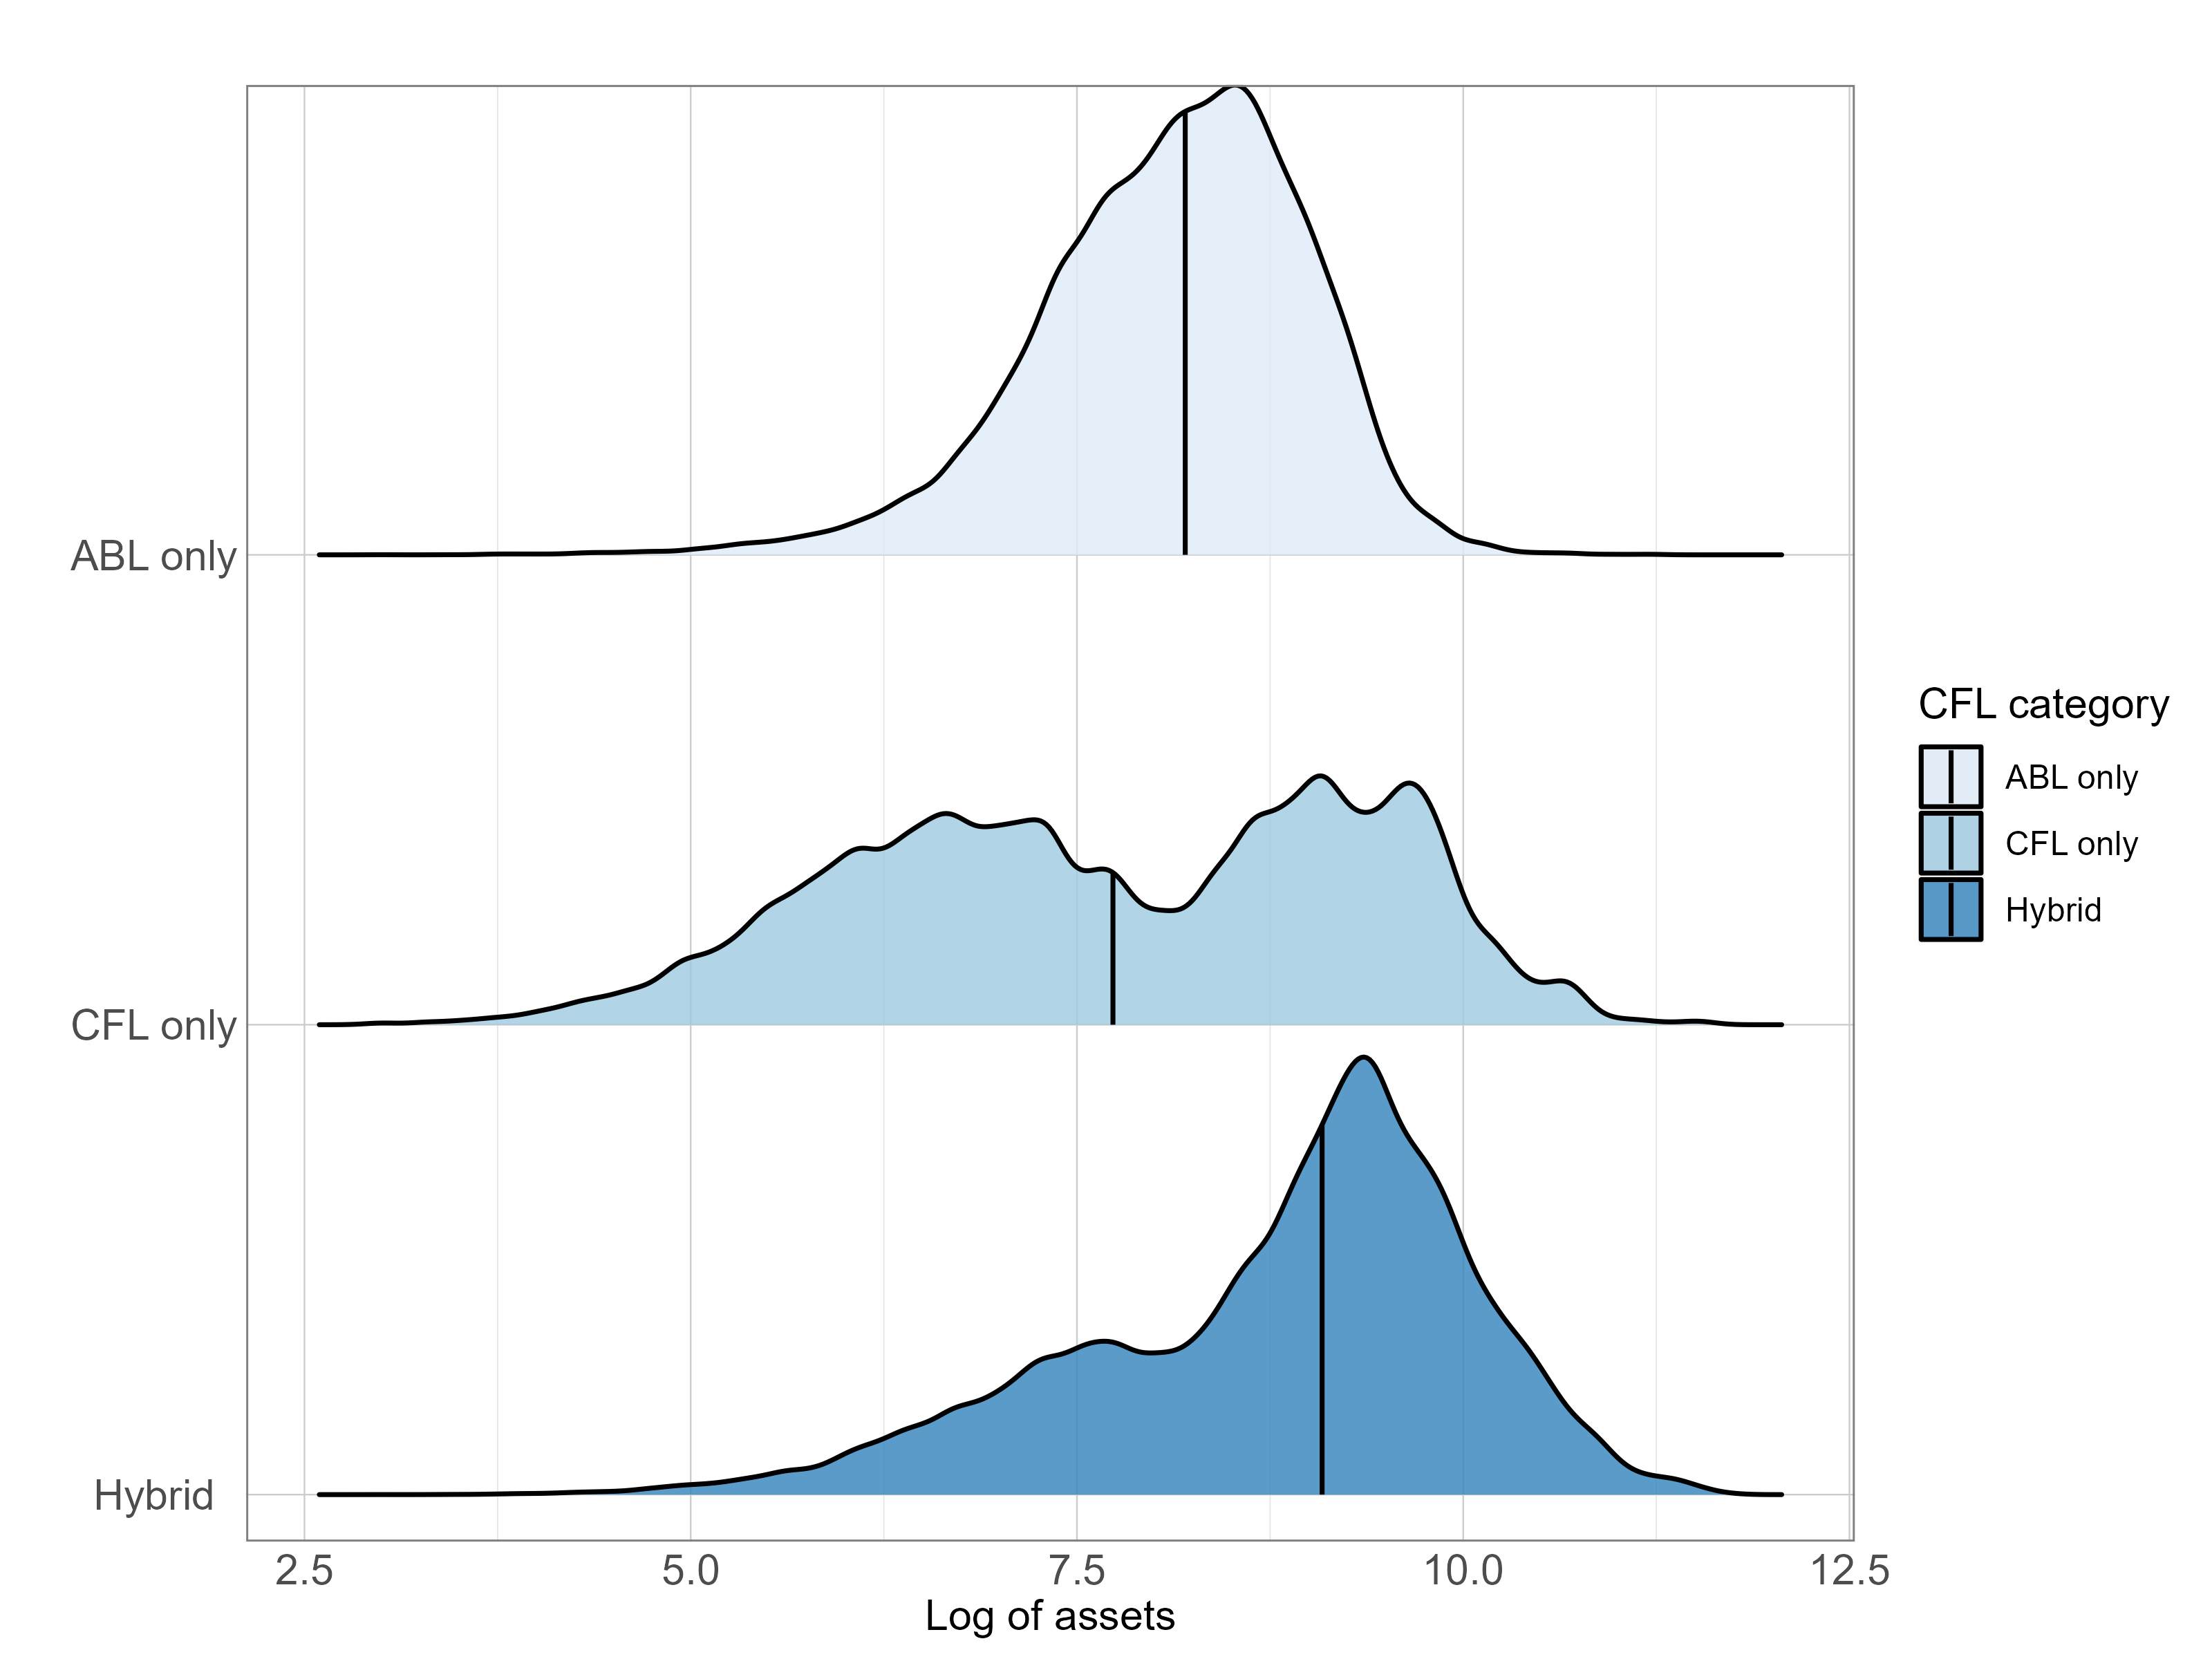
\includegraphics[width=0.8\textwidth]{ridges.png}
\end{figure}
\begin{center}
\hyperlink{slide2}{\beamerreturnbutton{back}}
\end{center}
\end{frame}

% ---------------------------------------------------------------------------------
\begin{frame}[label=U_country]{U-shape across countries}
\begin{figure}[H]  % [h] indicates placing the image here
    \centering
    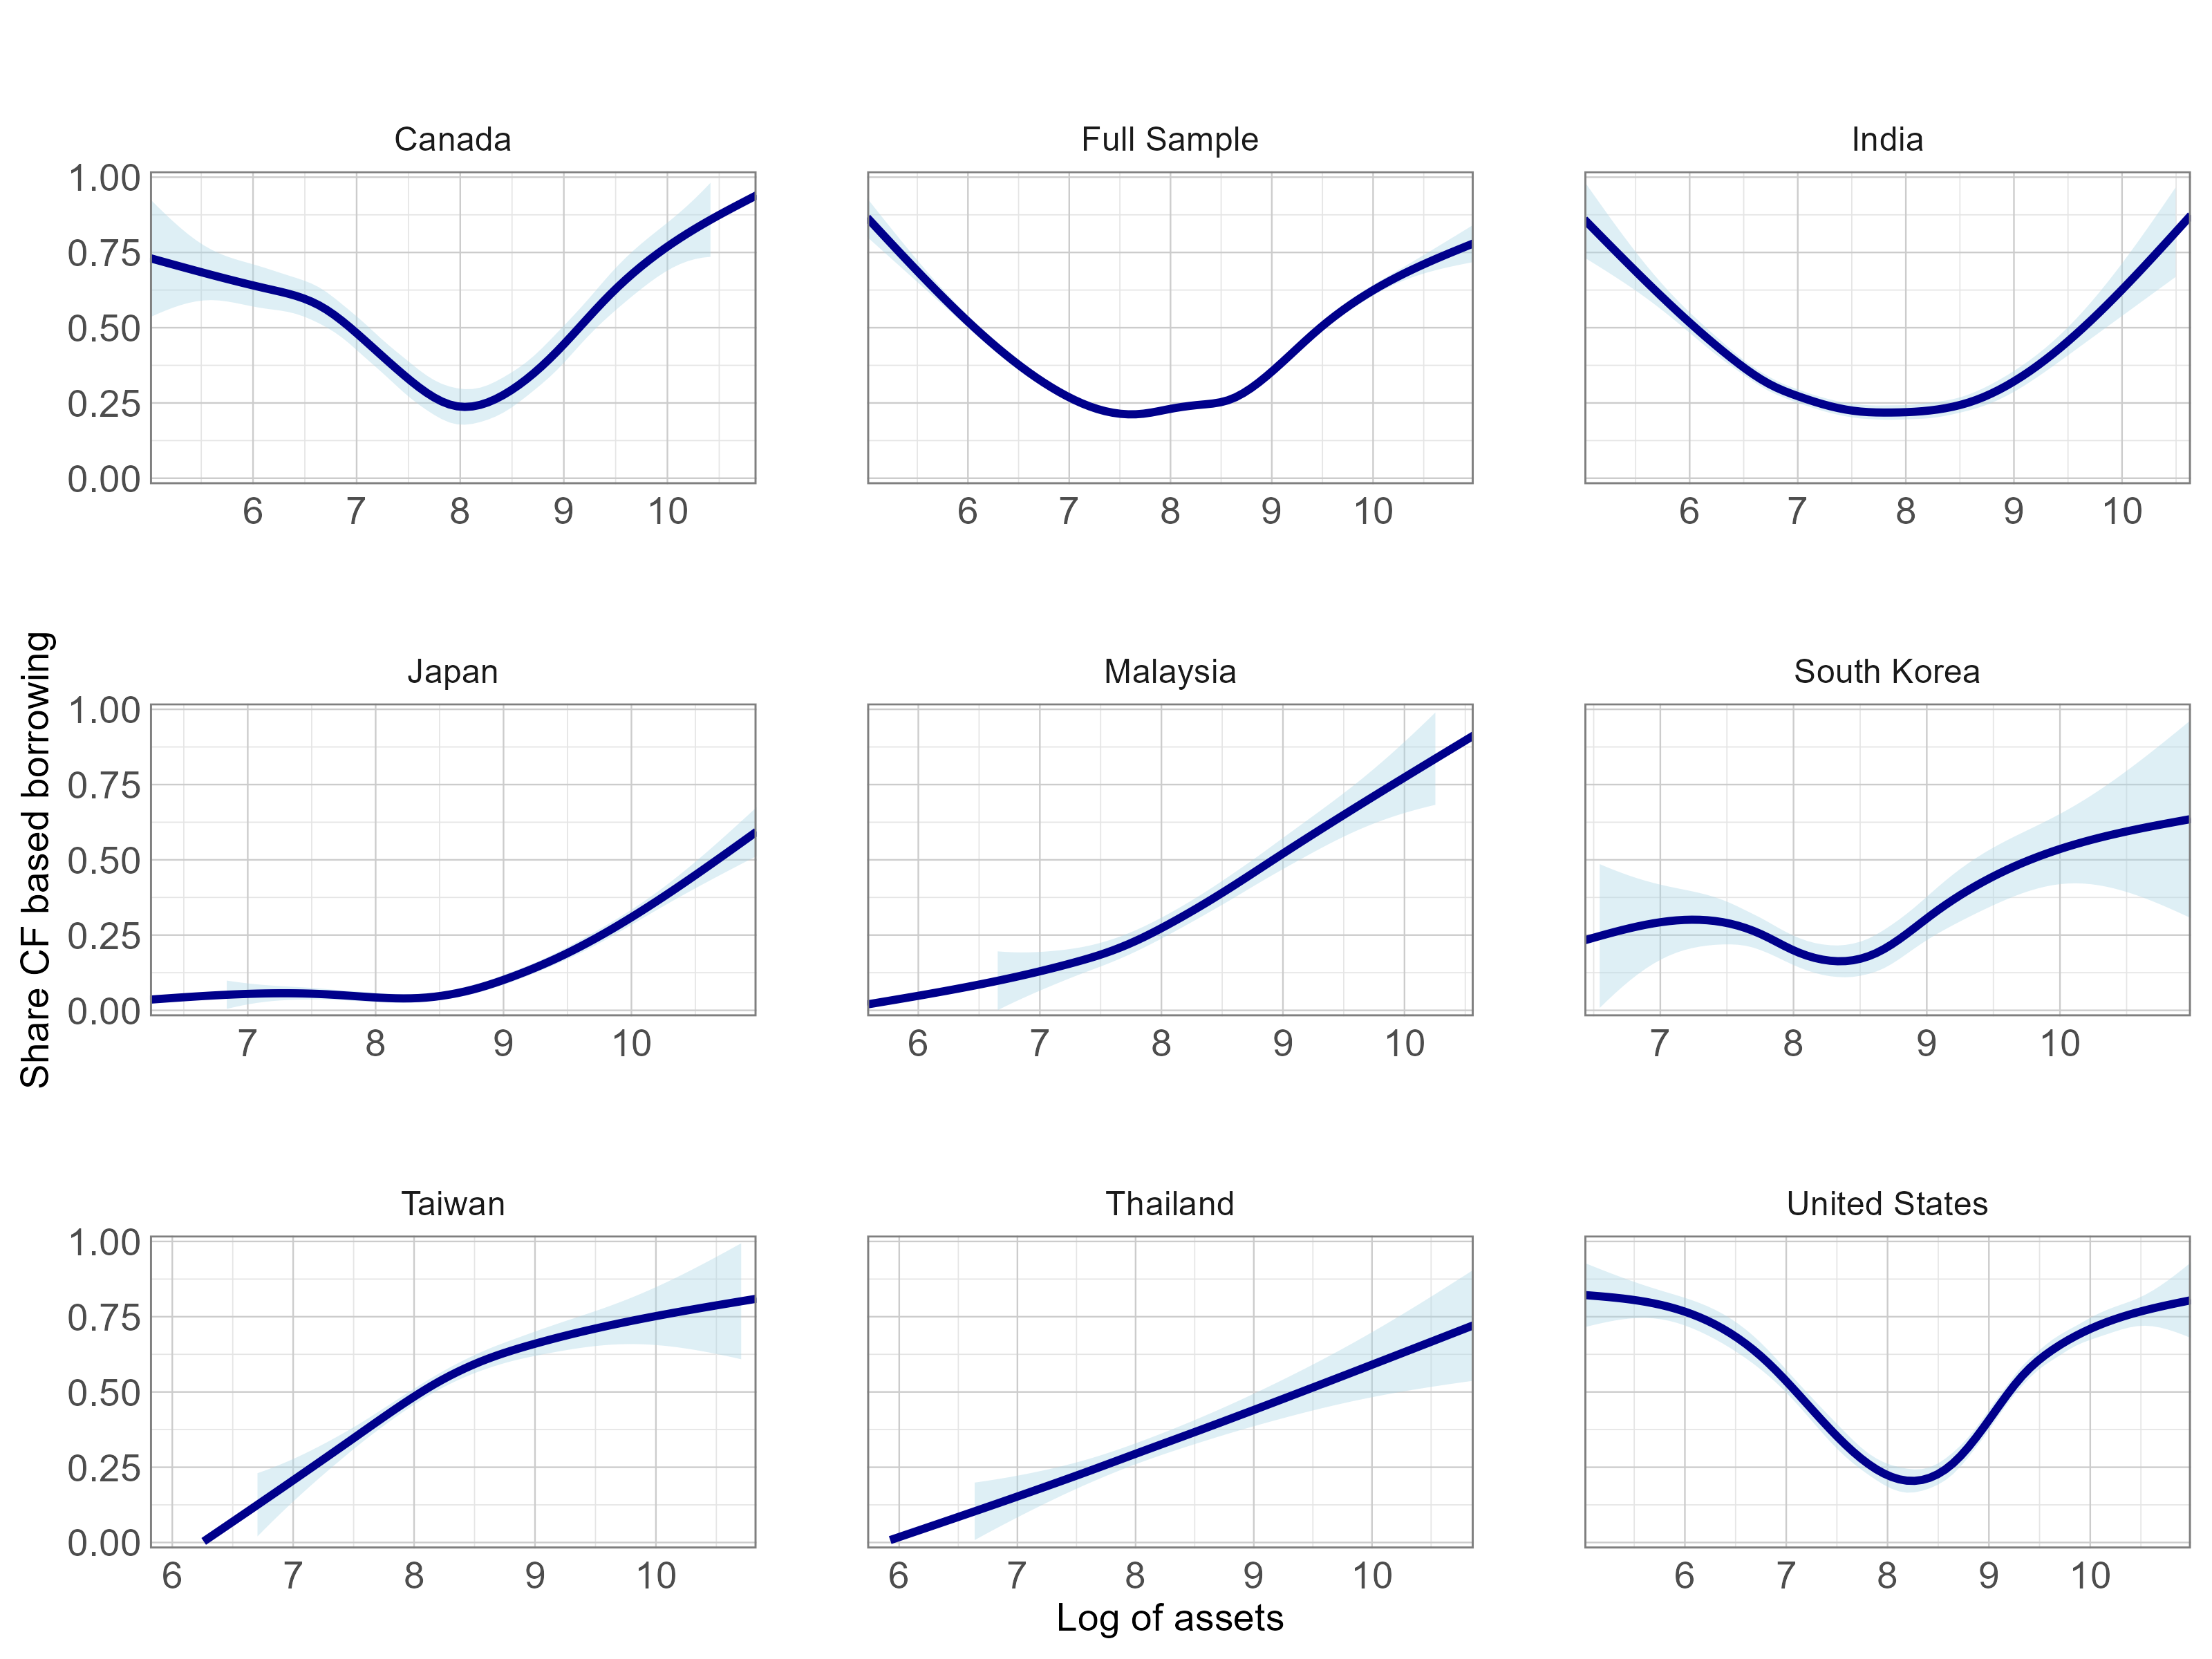
\includegraphics[width=0.8\textwidth]{presentations/smoothy_country.png}
\end{figure}
\begin{center}
\hyperlink{slide3}{\beamerreturnbutton{back}}
\end{center}
\end{frame}

% ---------------------------------------------------------------------------------
\begin{frame}[label=U_sector]{U-shape across sectors}
\begin{figure}[H]  % [h] indicates placing the image here
    \centering
    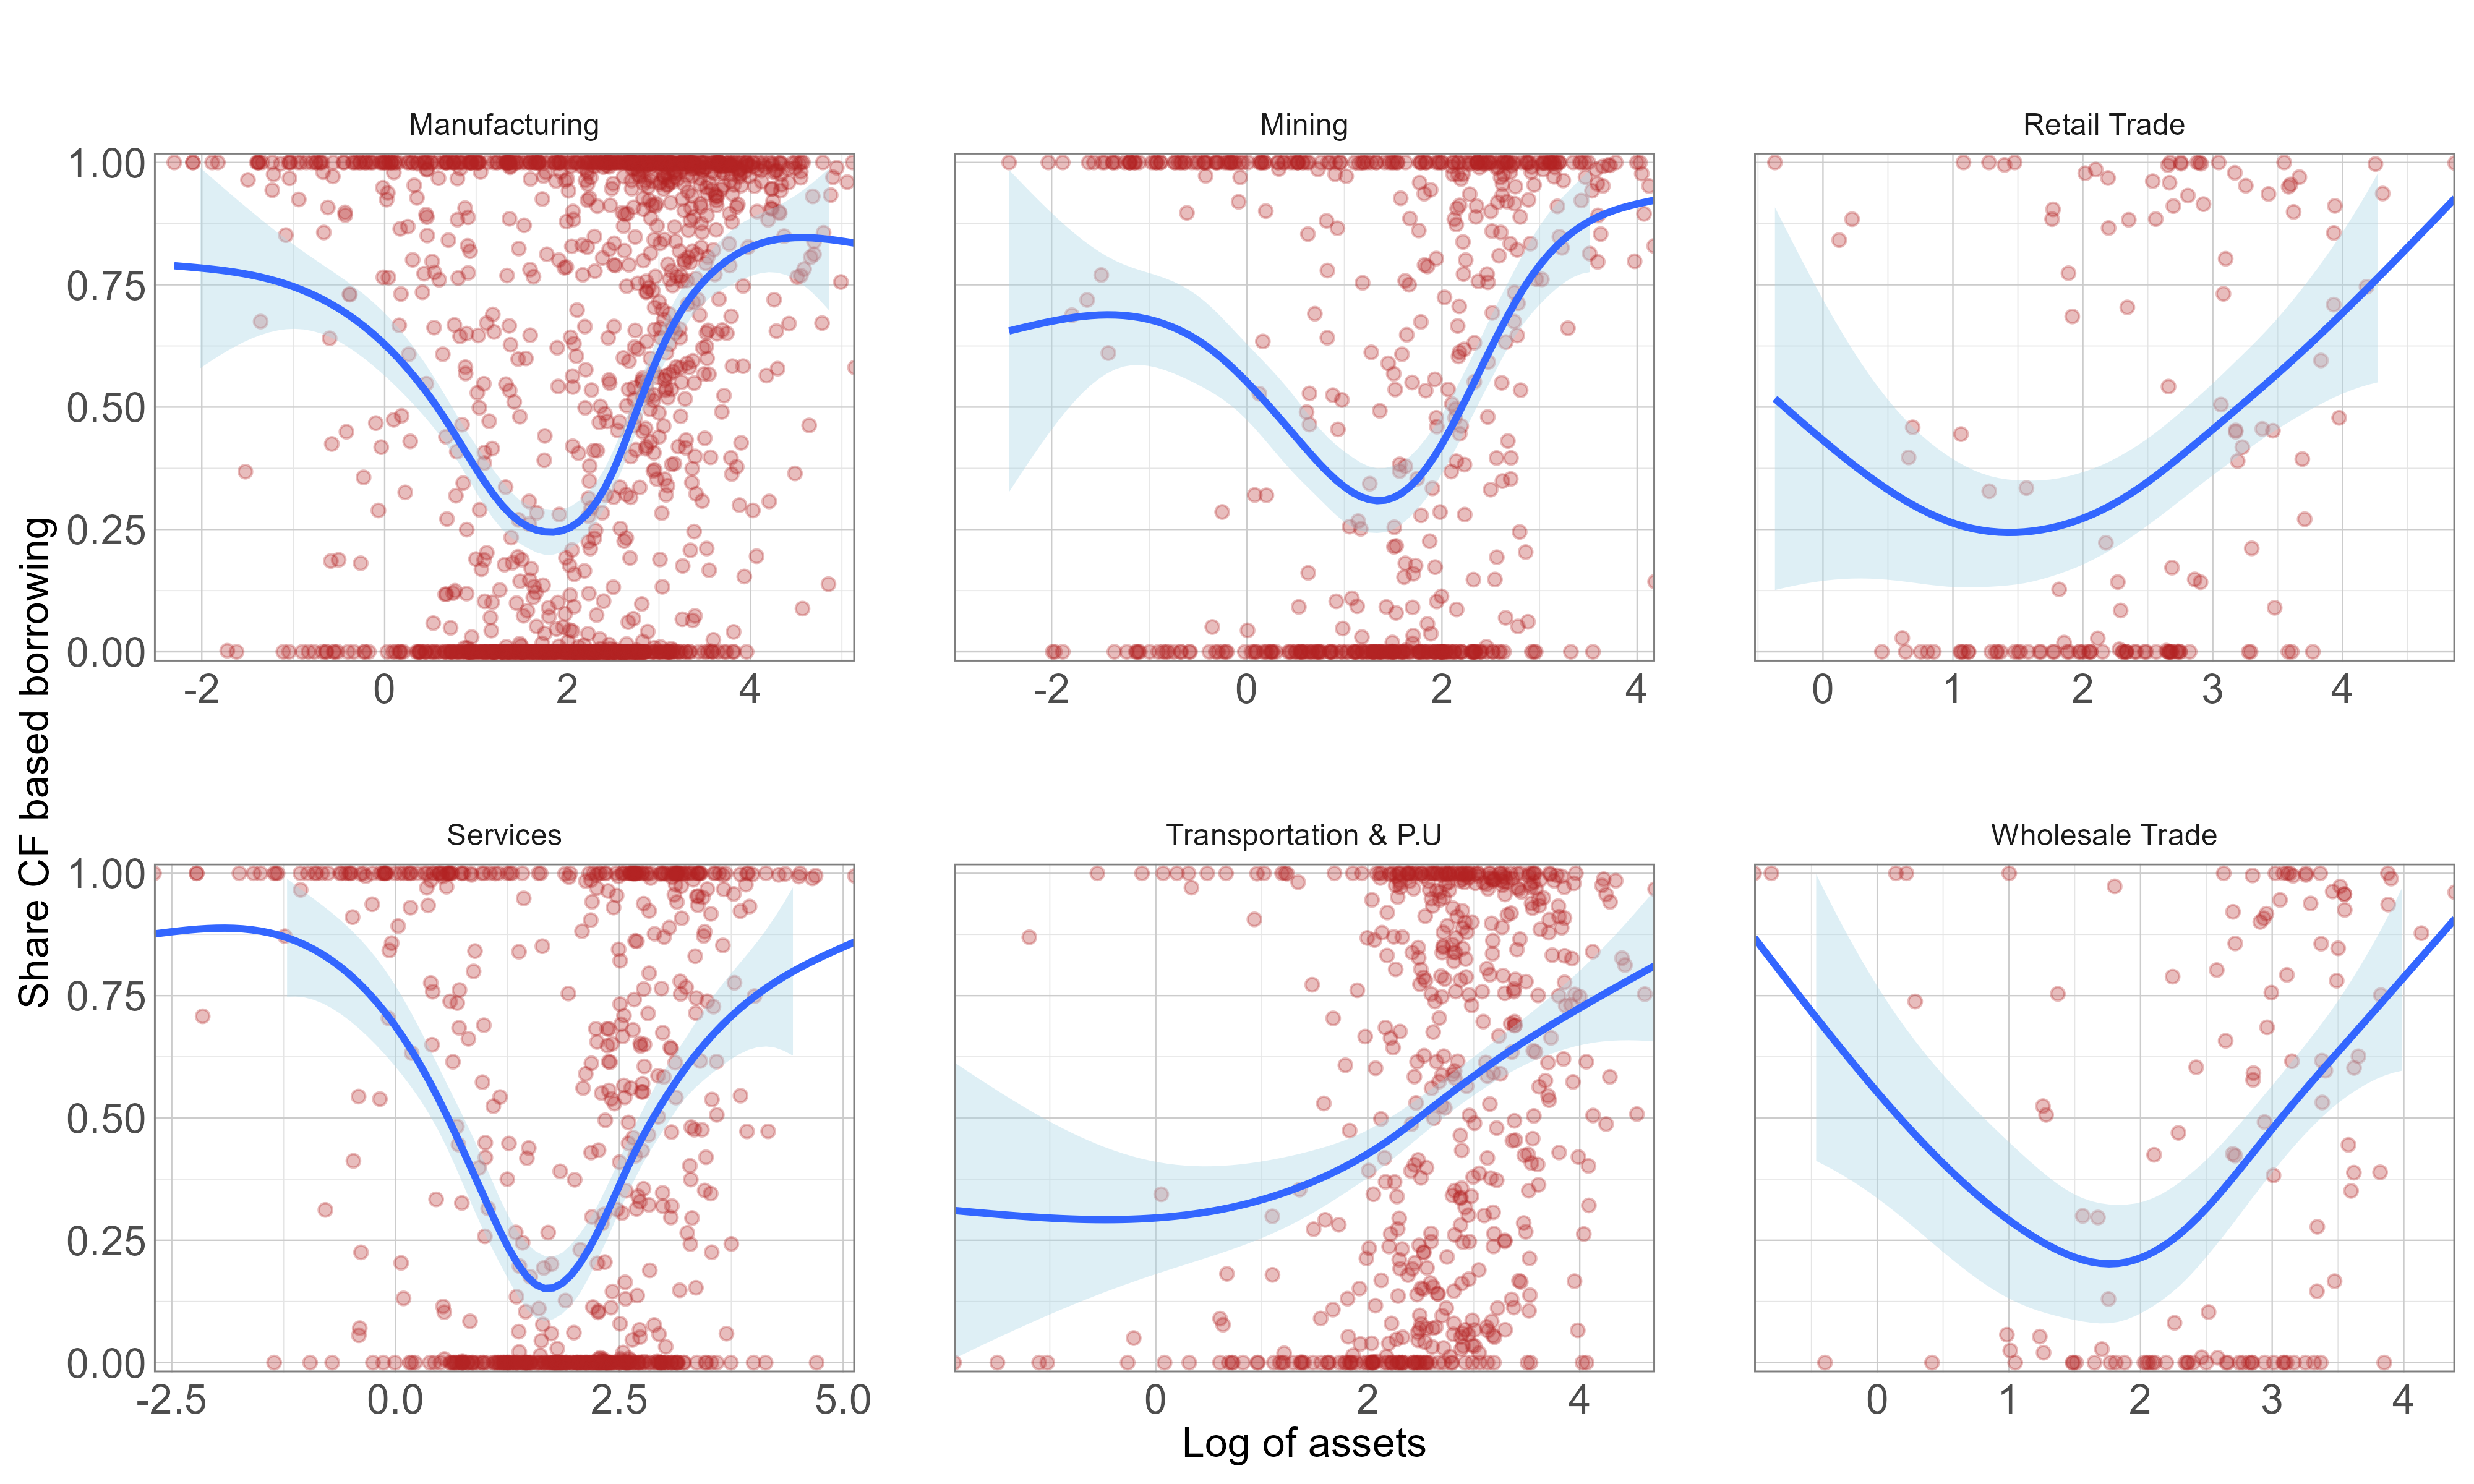
\includegraphics[width=0.9\textwidth]{presentations/smoothy1.png}
\end{figure}
\begin{center}
\hyperlink{slide3}{\beamerreturnbutton{back}}
\end{center}
\end{frame}


%------------------------------------------------
\begin{frame}[label = multi] \frametitle{Multivariate analysis}

\begin{table}[H]
\centering
\label{tab:your_table_label}
\resizebox{0.8\textwidth}{!}{%
\begin{tabular}{lcccccccc}
\toprule
& \multicolumn{3}{c}{POLS} & \multicolumn{3}{c}{FE regression} & \multicolumn{2}{c}{Firm level regression} \\
\cmidrule(lr){2-4} \cmidrule(lr){5-7} \cmidrule(lr){8-9}
LHS: CFL share & Value & SE & & Value & SE & & Value & SE \\
\midrule
Leverage & 0.176*** & (0.00662) & & 0.206*** & (0.0150) & & 0.244*** & (0.0155) \\
Pledgeability & -0.161*** & (0.0101) & & -0.174*** & (0.0297) & & -0.129*** & (0.0225) \\
Liquidity & 0.157*** & (0.0174) & & 0.0129 & (0.0256) & & -0.139*** & (0.0297) \\
Age & 0.00038*** & (4.96e-05) & &  -0.011*** & (0.0014)  & & 0.00057*** & (0.000126) \\
Log of employees & -0.0118*** & (0.00229) & & 0.00753 & (0.00753) & & -0.00238 & (0.00470) \\
Log of revenue & -0.000854 & (0.00293) & & 0.00326 & (0.00391) & & 0.00184 & (0.00453) \\
Log of assets & -1.059*** & (0.0289) & & -0.550*** & (0.0987) & & -1.321*** & (0.0647) \\
Log of assets squared & 0.0701*** & (0.00168) & & 0.0353*** & (0.00588) & & 0.0835*** & (0.00397)\\
Profitability & -0.44*** & (0.035) & & 0.035 & (0.033) & & -0.225*** & (0.059) \\
Productivity & 0.511*** & (0.0757) & & & & & 0.562*** & (0.200) \vspace{3mm} \\
Industry dummies & \textbf{X} & & & & & & \textbf{X} \\
Country dummies & \textbf{X} & & &  & & & \textbf{X} \\
Credit rating dummies & \textbf{X} & & &  & & &  \vspace{3mm}\\
Observations & 38,416 & & & 118,796 & & & 5,813 & \\
R-squared & 0.261 & & & 0.041 & & & 0.295 & \\
\bottomrule
\multicolumn{9}{c}{*** p$<$0.01, ** p$<$0.05, * p$<$0.1} \\
\end{tabular}%
}
\end{table}

\end{frame}

% -------------------------------------------------------
\begin{frame}[label=2dim]{2 dimensional relationships}
\begin{figure}[H]  % [h] indicates placing the image here
    \centering
    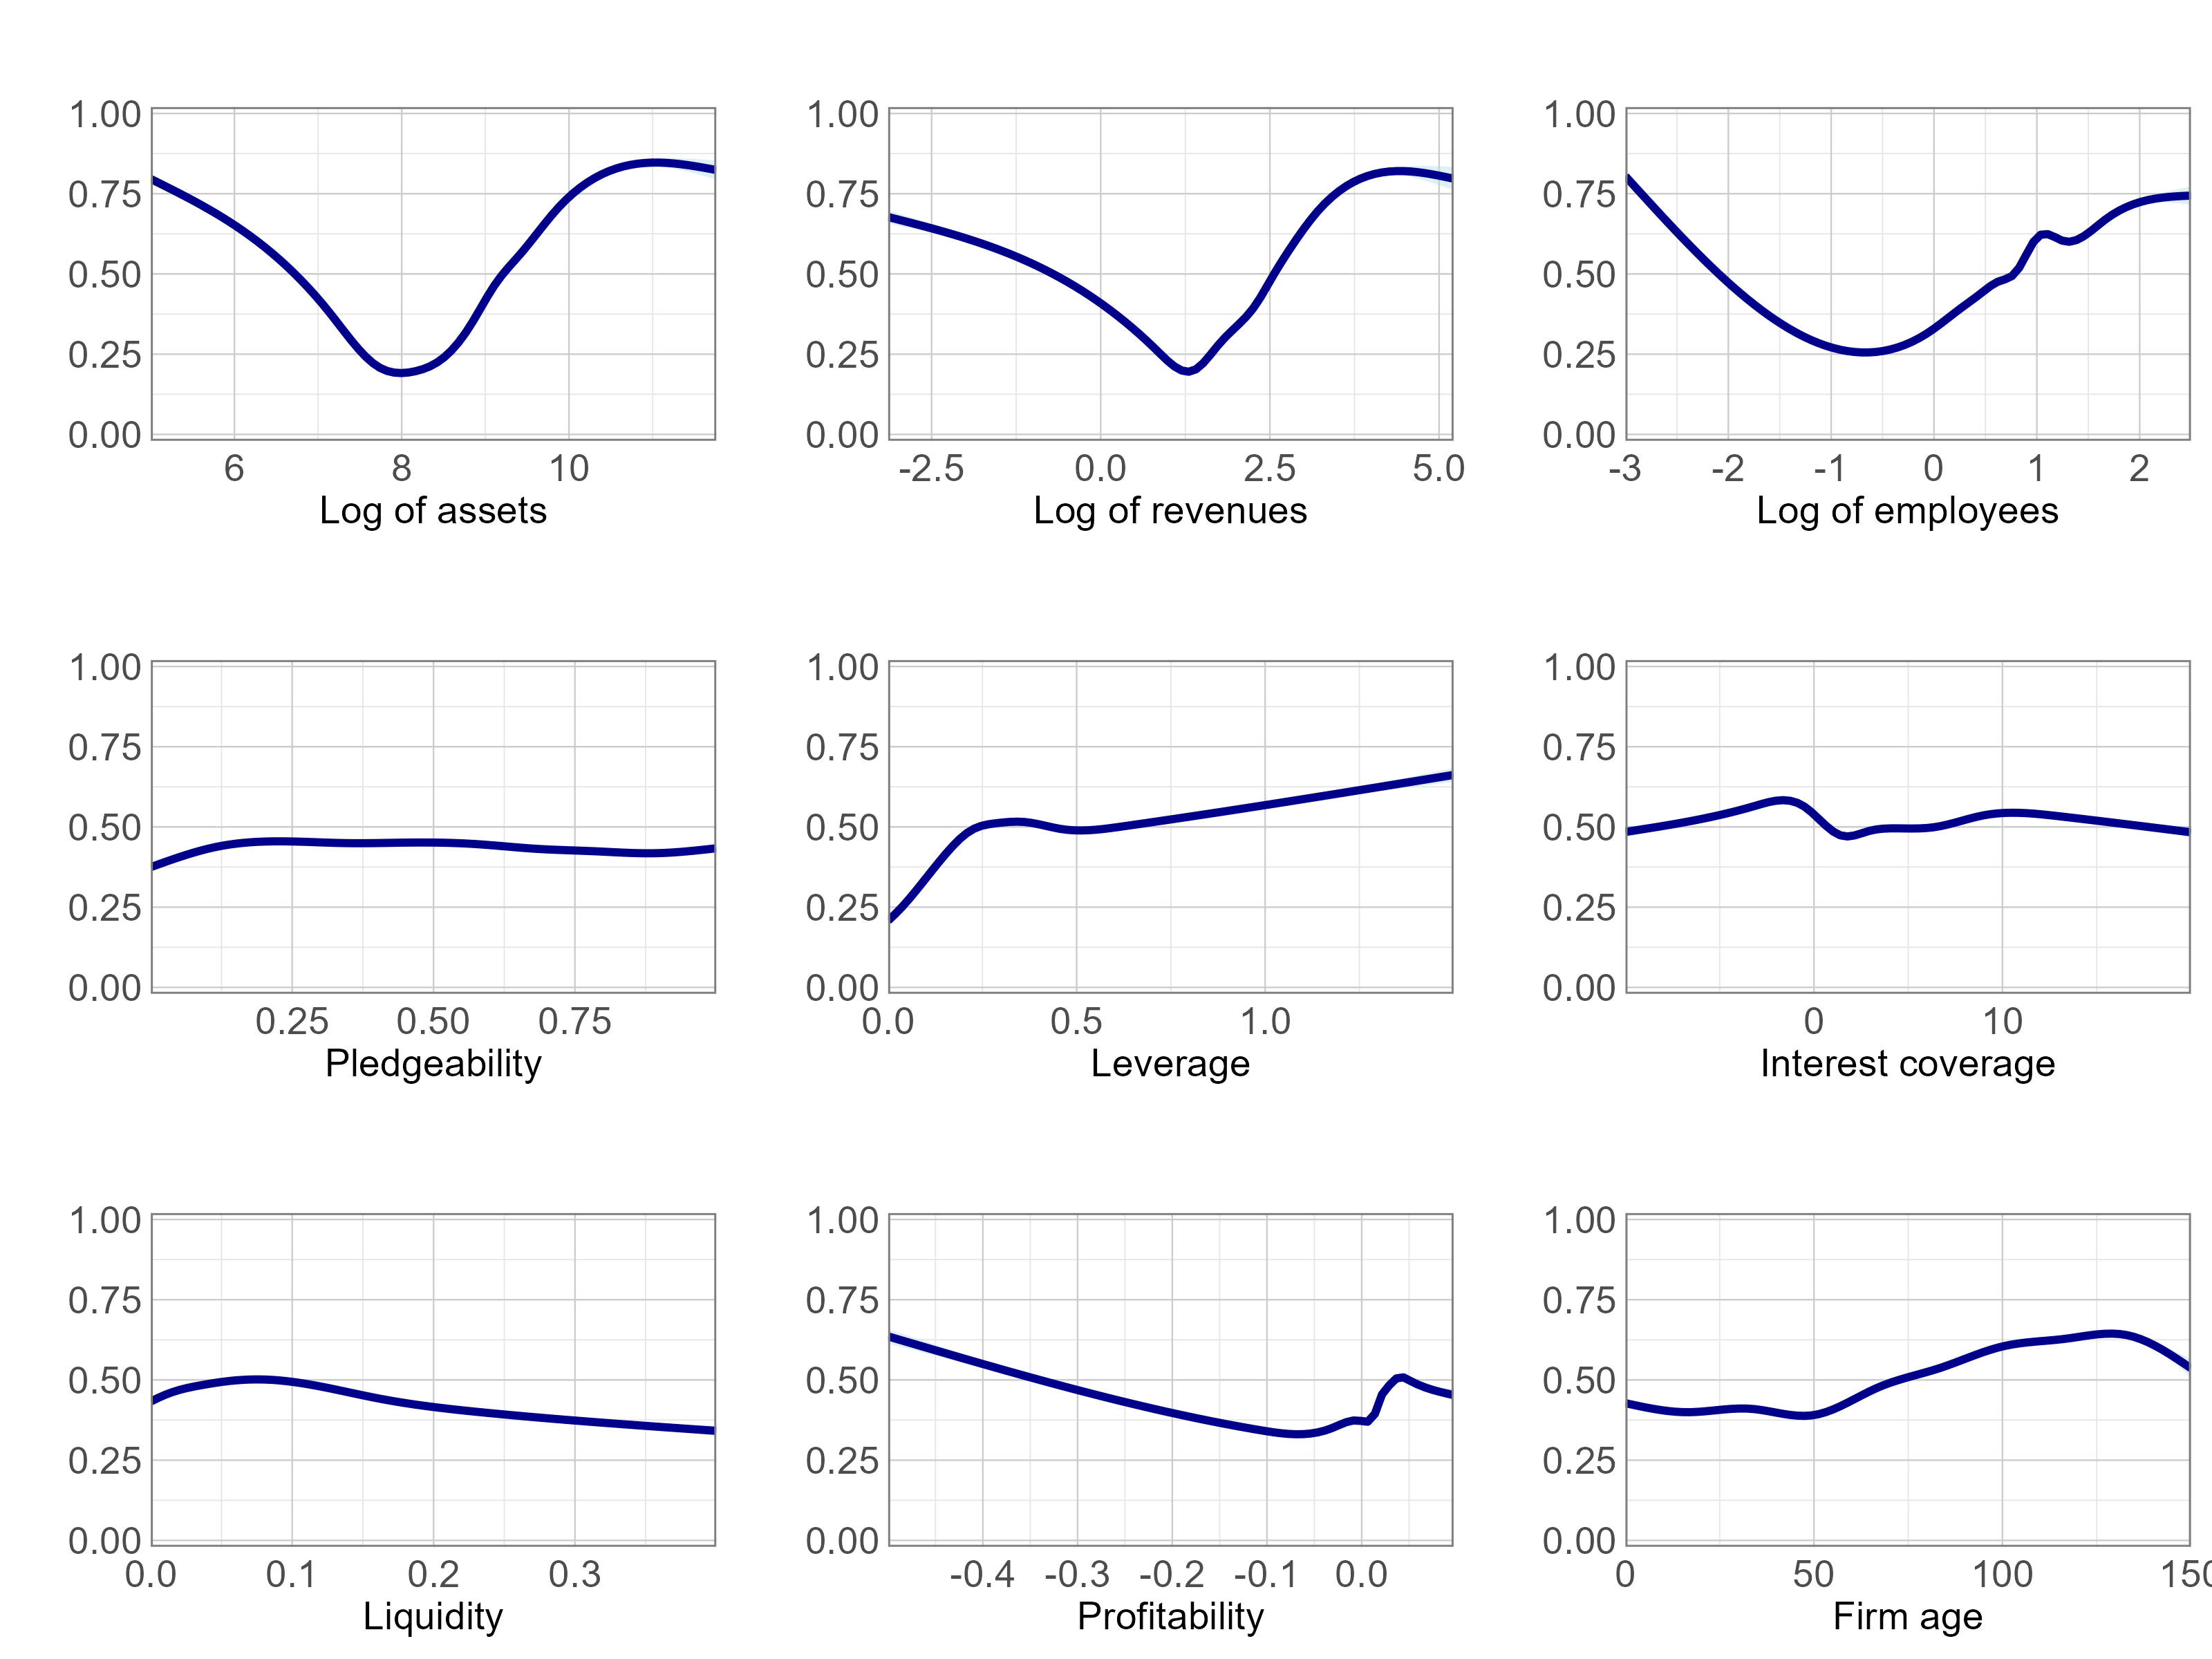
\includegraphics[width=0.73\textwidth]{presentations/varCFL.png}
\end{figure}
\restoregeometry % Restore the default page layout
\begin{center}
\hyperlink{nameit}{\beamerreturnbutton{back}}
\end{center}

\end{frame}


\end{document}
